\documentclass[11pt,letterpaper]{article}
\usepackage[margin=2.35cm,headheight=15pt]{geometry}
\usepackage[T1]{fontenc}
\usepackage{lmodern}
\usepackage[spanish,es-nodecimaldot]{babel}
\usepackage{graphicx,booktabs,tabularx,array,xcolor,fancyhdr,titlesec,enumitem,hyperref,caption,float,tikz,listings}
\usetikzlibrary{arrows.meta,positioning,babel}
\definecolor{RoadGreen}{HTML}{164B3B}
\definecolor{RoadTeal}{HTML}{197A89}
\definecolor{RoadBlue}{HTML}{245A8D}
\definecolor{RoadLight}{HTML}{EDF4F0}
\hypersetup{colorlinks=true,linkcolor=RoadBlue,urlcolor=RoadTeal,
  pdftitle={Proyecto de Sistemas Embebidos: Interfaz de bus CAN},
  pdfauthor={Roderic David Munguia Calvillo}}
\pagestyle{fancy}\fancyhf{}
\fancyhead[L]{\small\sffamily RoadLink}
\fancyhead[R]{\small\sffamily Interfaz de bus CAN}
\fancyfoot[C]{\small\sffamily\thepage}
\renewcommand{\headrulewidth}{0.4pt}
\renewcommand{\headrule}{\hbox to\headwidth{\color{RoadTeal}\leaders\hrule height \headrulewidth\hfill}}
\titleformat{\section}{\Large\bfseries\sffamily\color{RoadGreen}}{\thesection}{0.7em}{}
\titleformat{\subsection}{\large\bfseries\sffamily\color{RoadTeal}}{\thesubsection}{0.7em}{}
\titlespacing*{\section}{0pt}{2.2ex plus 0.8ex}{1.0ex}
\titlespacing*{\subsection}{0pt}{1.7ex plus 0.5ex}{0.7ex}
\setlist[itemize]{leftmargin=1.5em,itemsep=0.25em,topsep=0.35em}
\renewcommand{\arraystretch}{1.22}
\newcolumntype{Y}{>{\raggedright\arraybackslash}X}
\emergencystretch=1.5em
\lstset{basicstyle=\ttfamily\small,backgroundcolor=\color{RoadLight},
  frame=single,framerule=0.3pt,rulecolor=\color{RoadTeal},
  xleftmargin=0.4em,xrightmargin=0.4em,aboveskip=0.7em,belowskip=0.7em,
  breaklines=true,showstringspaces=false}
\begin{document}
\begin{titlepage}
  \pagecolor{RoadLight}
  \begin{center}
    \vspace*{1.0cm}
    {\sffamily\bfseries\fontsize{20}{24}\selectfont\color{RoadTeal} ROADLINK}\par
    \vspace{0.35cm}
    {\color{RoadTeal}\rule{0.82\textwidth}{2.2pt}}\par
    \vfill
    {\sffamily\bfseries\fontsize{28}{34}\selectfont\color{RoadGreen} Proyecto de Sistemas Embebidos}\par
    \vspace{0.35cm}
    {\sffamily\bfseries\fontsize{38}{44}\selectfont\color{RoadBlue} Interfaz de bus CAN}\par
    \vspace{0.8cm}\vfill
    \begin{tabular}{>{\sffamily\bfseries}r >{\sffamily}l}
      Autor: & Roderic David Munguia Calvillo \\
      Proyecto: & RoadLink \\
      Fecha: & 29 de septiembre de 2026 \\
    \end{tabular}
    \vfill
    \begin{minipage}{0.82\textwidth}\centering
      \colorbox{RoadGreen}{\parbox{0.94\textwidth}{\centering\color{white}\sffamily\small
        Enlace entre el ESP32, el MCP2515 y la red del vehículo}}
    \end{minipage}
    \vspace*{0.8cm}
  \end{center}
\end{titlepage}
\nopagecolor
\pagenumbering{roman}
\tableofcontents
\begin{thebibliography}{3}
\bibitem{mcp2515} Microchip Technology, \emph{MCP2515 Stand-Alone CAN Controller
with SPI Interface Data Sheet}, \href{https://ww1.microchip.com/downloads/en/DeviceDoc/MCP2515-Stand-Alone-CAN-Controller-with-SPI-20001801J.pdf}{hoja de datos}.
\bibitem{canfisica} Microchip Technology, \emph{A CAN Physical Layer Discussion},
\href{https://www.microchip.com/en-us/application-notes/an228}{nota de aplicación AN228}.
\bibitem{obd} CSS Electronics, \emph{OBD2 Explained},
\href{https://www.csselectronics.com/pages/obd2-explained-simple-intro}{guía del conector y CAN}.
\end{thebibliography}
\clearpage\pagenumbering{arabic}

\section{Introducción}
La interfaz CAN permite que RoadLink observe las tramas presentes en la red
vehicular y, cuando una función lo requiere, envíe solicitudes de diagnóstico.
\textbf{CAN} describe el intercambio de tramas en el bus; \textbf{OBD-II} es una
aplicación de diagnóstico que utiliza ese enlace en vehículos compatibles. No
son el mismo módulo ni toda trama CAN contiene una lectura OBD-II.

El ESP32 no se conecta directamente a los dos cables del vehículo. En este
montaje se comunica por SPI con un controlador MCP2515; la parte física del
módulo CAN adapta sus señales a CAN-H y CAN-L. El documento distingue lo
confirmado por el firmware, las lecturas visibles en las fotografías de prueba
y aquello que todavía falta verificar con mediciones o registros originales.

\section{Recorrido de la señal y conexión}
La ruta funcional parte del ESP32, pasa por el bus SPI y el MCP2515, continúa
por el transceptor del módulo CAN y termina en el conector OBD-II. Para CAN de
alta velocidad, los contactos habituales del conector son el \textbf{pin 6
(CAN-H)} y el \textbf{pin 14 (CAN-L)} \cite{obd}. La alimentación que también se
toma de OBD-II se documenta aparte, en el informe de la interfaz de
alimentación. El módulo CAN pertenece a la rama general de 5 V del prototipo.

\begin{figure}[H]\centering
  \begin{tikzpicture}[>=Latex,
    block/.style={draw=RoadTeal,fill=RoadLight,rounded corners=2pt,
      minimum height=1.05cm,text width=2.4cm,align=center,font=\small\sffamily},
    arr/.style={-{Latex[length=2mm]},thick,color=RoadBlue}]
    \node[block] (esp) at (0,0) {ESP32\\programa RoadLink};
    \node[block] (mcp) at (3.5,0) {MCP2515\\controlador CAN};
    \node[block] (phy) at (7.0,0) {Transceptor\\capa física CAN};
    \node[block] (obd) at (10.5,0) {Conector OBD-II\\CAN-H y CAN-L};
    \draw[arr] (esp) -- (mcp);
    \draw[arr] (mcp) -- (phy);
    \draw[arr] (phy) -- (obd);
  \end{tikzpicture}
  \caption{Cadena funcional de la interfaz CAN; no representa la posición ni
  la longitud real de las pistas de la PCB.}\label{fig:cadena}
\end{figure}

\begin{figure}[H]\centering
  \begin{minipage}[c]{0.59\textwidth}
    El MCP2515 es un controlador CAN externo con interfaz SPI \cite{mcp2515}.
    Forma y recibe las tramas; el transceptor de la placa CAN adapta las
    señales al par diferencial. El conector OBD-II es el enchufe de esa ruta,
    no el transceptor. La foto muestra cómo se instaló en RoadLink, pero no
    permite comprobar el contacto interno de los pines 6 y 14 ni identificar
    el transceptor de la placa CAN.
  \end{minipage}\hfill
  \begin{minipage}[c]{0.34\textwidth}\centering
    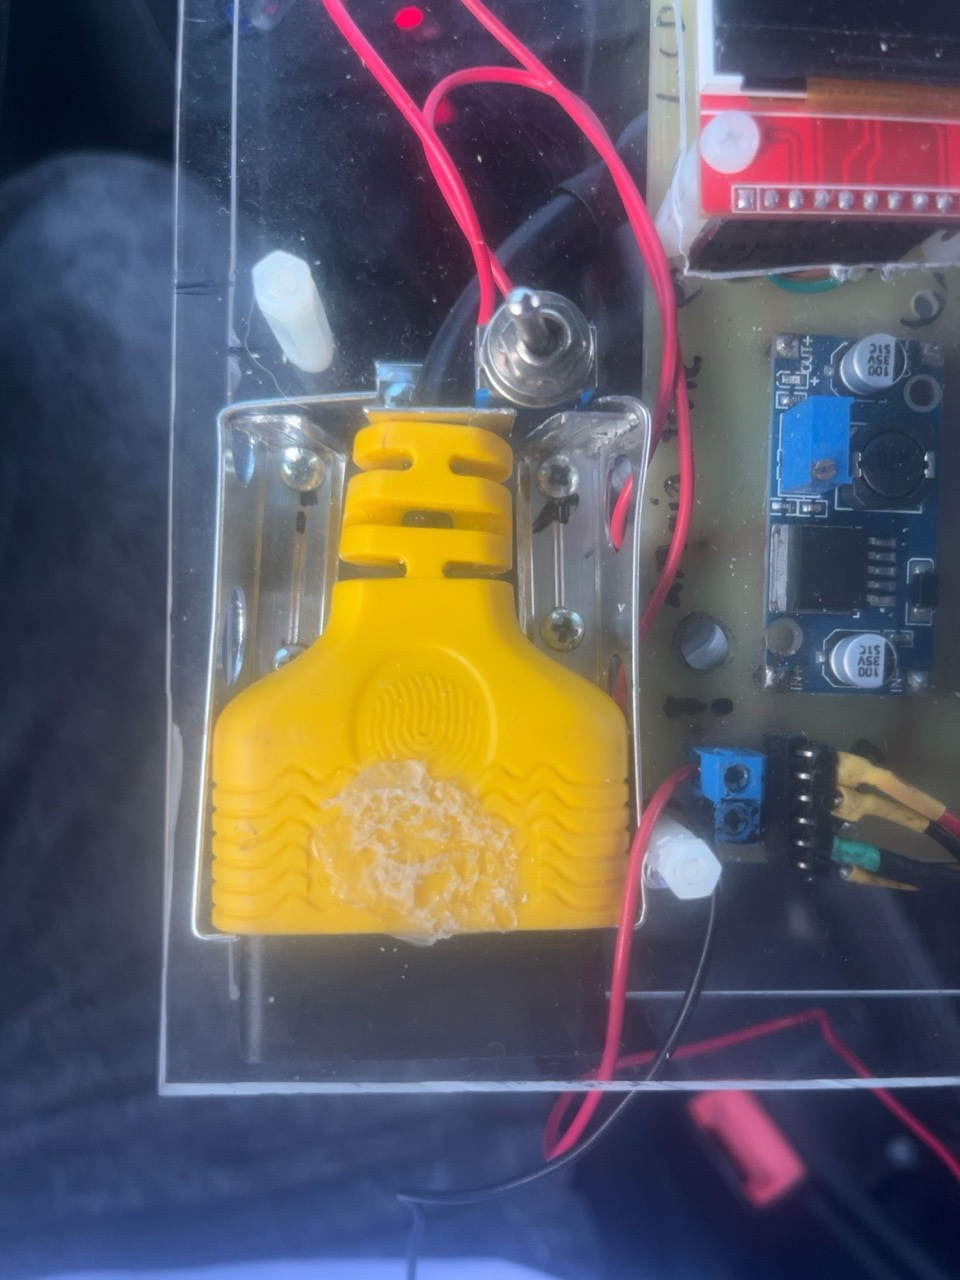
\includegraphics[width=\linewidth,height=4.6cm,keepaspectratio]{../../recursos/imagenes/conector-obd2-montaje-roadlink.jpg}
  \end{minipage}
  \caption{Conector OBD-II montado en RoadLink. Fotografía del autor, sin fecha
  de toma registrada; no verifica por sí sola el pinout.}
  \label{fig:conector}
\end{figure}

\subsection{Pines del ESP32 y SPI compartido}
El archivo \texttt{AppConfig.h} registra la asignación usada por el firmware.
La pantalla TFT comparte reloj y datos SPI con el MCP2515; cada periférico
tiene su propia selección de chip. La línea INT se reserva en GPIO 4, aunque
el servicio actual consulta la recepción durante su ciclo de actualización y
no instala una rutina de interrupción.

\begin{table}[H]\centering
  \caption{Conexiones CAN declaradas en el firmware de RoadLink.}
  \begin{tabularx}{\textwidth}{>{\bfseries}p{2.2cm} >{\centering\arraybackslash}p{1.5cm} Y}
    \toprule Señal & GPIO & Función \\
    \midrule
    CS & 23 & Selecciona el MCP2515 en el bus SPI. \\
    SO / MISO & 19 & Datos del MCP2515 hacia el ESP32. \\
    SI / MOSI & 18 & Datos del ESP32 hacia el MCP2515. \\
    SCK & 5 & Reloj SPI compartido con la TFT. \\
    INT & 4 & Salida de interrupción del módulo; configurada como entrada. \\
    \bottomrule
  \end{tabularx}
\end{table}

La alimentación de 5 V de la placa CAN no demuestra que todas sus señales
SPI sean compatibles directamente con los GPIO de 3,3 V del ESP32. La
adaptación de niveles y la tensión real en SO/INT deben verificarse en el
montaje. Tampoco se supone que el módulo añada o requiera una resistencia de
terminación concreta: depende de la placa y de la red \cite{canfisica}.

\section{Comportamiento implementado en el firmware}
\texttt{CanService} inicia el MCP2515 con el oscilador configurado en
\textbf{8 MHz}. La velocidad predeterminada es \textbf{500 kbit/s} y el
arranque predeterminado es \textbf{Listen-only}: recibe sin emitir tramas. El
menú permite seleccionar 125, 250, 500 kbit/s o 1 Mbit/s. La velocidad
inicial es un ajuste de firmware, no una medición ni una propiedad universal
de todos los vehículos.

\begin{lstlisting}[caption={Fragmento de inicialización de \texttt{CanService.cpp}.}]
initializationResult_ = controller_.begin(
    MCP_ANY, libraryBitrate(bitrate), MCP_8MHZ);
initialized_ = initializationResult_ == CAN_OK;
\end{lstlisting}

En cada ciclo, \texttt{CanService} lee las tramas disponibles, conserva la
última, contabiliza tramas por segundo e identifica los IDs observados. El
límite de procesamiento es de 48 tramas por vuelta para no monopolizar el
programa. La transmisión únicamente se permite cuando el controlador se
inicializó y se cambió al modo \textbf{Normal}; en Listen-only se rechaza.
Así, observar el bus y consultar una ECU son acciones distintas.

\section{Relación con OBD-II}
\texttt{ObdService} utiliza \texttt{CanService} para formar solicitudes
diagnósticas ISO 15765-4 con identificadores estándar de 11 bits. El código
emplea \texttt{0x7DF} como solicitud funcional y acepta respuestas
\texttt{0x7E8--0x7EF}. Para mensajes mayores de una trama, reúne segmentos
ISO-TP y envía control de flujo. Incluye descubrimiento de ECUs, datos en
vivo, PIDs admitidos, códigos de falla y VIN. El borrado de códigos requiere
confirmación en la interfaz: modifica información del vehículo y no es una
lectura pasiva.

\begin{lstlisting}[caption={Formación de una solicitud OBD-II en el código actual.}]
uint8_t frame[8] = {};
frame[0] = payloadLength;
for (uint8_t index = 0; index < payloadLength; ++index) {
  frame[index + 1] = payload[index];
}
return can_.sendFrame(requestId, false, 8, frame);
\end{lstlisting}

Estas consultas requieren modo Normal: una ECU no puede responder a una
solicitud que RoadLink nunca transmitió. Las fotografías de la siguiente
sección documentan pantallas de uso, aunque no sustituyen una traza de las
tramas intercambiadas.

\section{Evidencia fotográfica de funcionamiento}

Las Figuras~\ref{fig:can-prueba} y \ref{fig:obd-prueba} muestran dos pantallas
del prototipo proporcionadas por el autor. No se conoce la fecha de captura,
el vehículo ni si ambas corresponden a la misma sesión. Por ello se registran
como \emph{lecturas mostradas por RoadLink}, no como mediciones independientes
ni como una secuencia temporal verificada.

\begin{figure}[H]\centering
  \begin{minipage}[t]{0.47\textwidth}\centering
    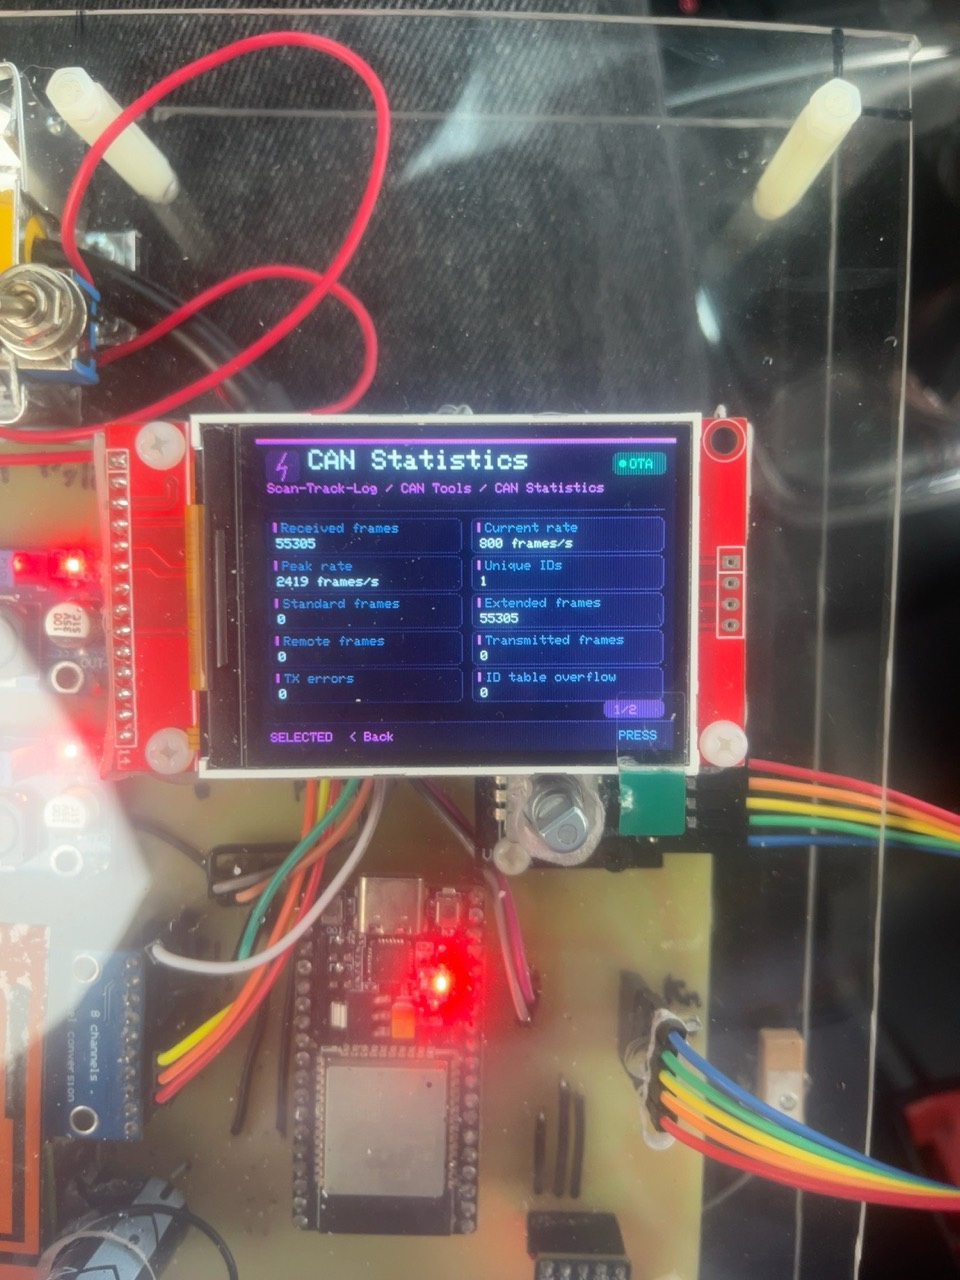
\includegraphics[width=\linewidth,height=7.5cm,keepaspectratio]{../../recursos/imagenes/can-estadisticas-pantalla-roadlink.jpg}
    \caption{Pantalla de estadísticas CAN del prototipo.}
    \label{fig:can-prueba}
  \end{minipage}\hfill
  \begin{minipage}[t]{0.47\textwidth}\centering
    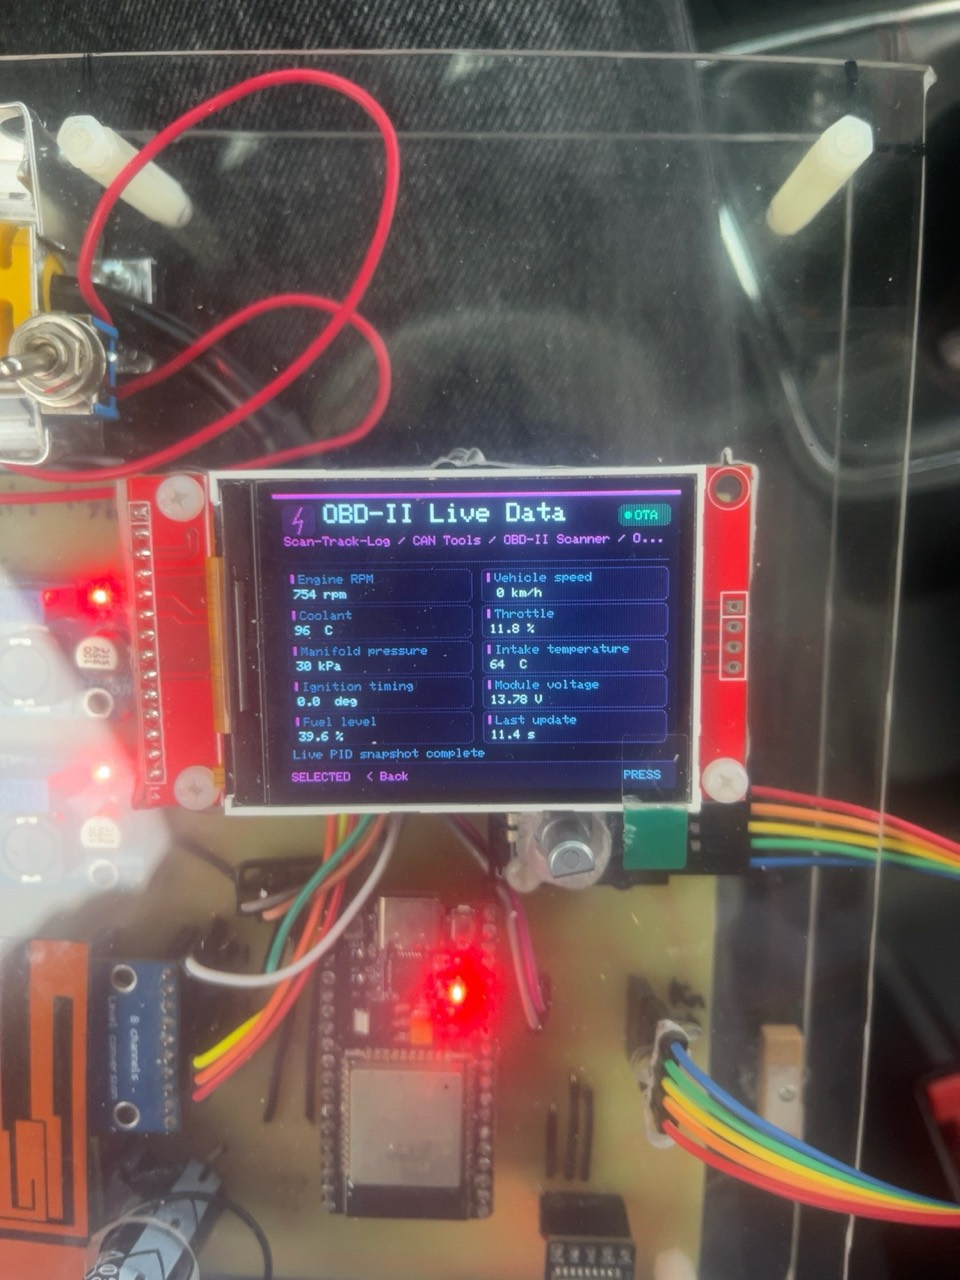
\includegraphics[width=\linewidth,height=7.5cm,keepaspectratio]{../../recursos/imagenes/obd2-datos-vivos-pantalla-roadlink.jpg}
    \caption{Pantalla de datos OBD-II del prototipo.}
    \label{fig:obd-prueba}
  \end{minipage}
\end{figure}

En la primera fotografía se leen \textbf{55\,305 tramas recibidas}, una tasa
actual de \textbf{800 tramas/s} y un máximo mostrado de \textbf{2\,419
tramas/s}. La pantalla registra un ID único, 55\,305 tramas extendidas,
ninguna estándar y cero tramas transmitidas, errores de transmisión o
desbordamientos de la tabla de IDs. Son contadores del firmware en ese
instante, no una caracterización completa de la red.

En la segunda fotografía aparece el mensaje ``Live PID snapshot complete''.
Entre los valores legibles figuran \textbf{754 rpm}, \textbf{0 km/h},
\textbf{96 $^\circ$C} de refrigerante, \textbf{11,8\,\%} de acelerador,
\textbf{30 kPa} de presión del colector, \textbf{13,78 V} de voltaje del
módulo y \textbf{39,6\,\%} de combustible. La pantalla indica además
``Last update 11.4 s''; por tanto, la foto no demuestra que esos valores se
estuvieran actualizando continuamente en el momento de tomarla.

La pantalla CAN muestra exclusivamente tramas \emph{extendidas}, mientras que
las solicitudes OBD-II descritas en el código usan identificadores estándar
de 11 bits. Sin fecha, configuración y traza de cada prueba, no corresponde
afirmar que ambas pantallas describen el mismo tráfico o que una explica a la
otra. Esta diferencia debe comprobarse en una sesión de prueba registrada.

\section{Comprobación y límites}
Las fotografías aportan evidencia de recepción CAN y de una pantalla OBD-II
con valores decodificados. Para completar la validación se requiere además:
\begin{itemize}
  \item alimentación, tierra común, niveles lógicos y continuidad del par
    CAN-H/CAN-L con el vehículo desconectado;
  \item arranque del MCP2515 a 8 MHz con la tasa correcta, y funcionamiento
    simultáneo de TFT y CAN en el SPI compartido;
  \item observación inicial en Listen-only, con registro de IDs, tramas por
    segundo y errores, sin atribuir significado a datos no decodificados;
  \item una consulta OBD-II de lectura en un entorno controlado, guardando la
    solicitud y la respuesta antes de presentarlas como evidencia experimental.
\end{itemize}

No se debe añadir terminación al bus del automóvil sin revisar la red y la
placa concreta. Una lectura fallida tampoco demuestra por sí sola un defecto
del MCP2515: pueden influir el protocolo admitido, el encendido del vehículo,
la tasa CAN, el cableado, los niveles lógicos o la alimentación. Las
mediciones del par, los registros originales de tramas y las condiciones de
las pruebas mostradas quedan pendientes de incorporarse como evidencias.

\section{Conclusiones}
RoadLink separa la adquisición CAN de la interpretación OBD-II. El ESP32
controla por SPI un MCP2515 y, mediante el transceptor del módulo, se
comunica con el par CAN vehicular. El arranque en Listen-only permite observar
sin transmitir; las consultas OBD-II requieren habilitar el envío. El firmware
ya define conexiones, velocidad inicial, modos y operaciones diagnósticas,
mientras que el pinout físico, la identificación del transceptor y las pruebas
fotografiadas deben ampliarse con registros y mediciones antes de declarar
validada por completo la interfaz.
\end{document}
